\documentclass[a4paper, 12pt]{report}

\setcounter{tocdepth}{3}
\setcounter{secnumdepth}{3}
% data visutalization
\usepackage{pgf-pie}
\usepackage{pgfplots}
\pgfplotsset{compat=1.18} 
% \hfuzz=15pt
%styling the doc
\linespread{2}
% \usepackage[none]{hyphenat} % prevent hyphenation
\usepackage[english]{babel}
\usepackage{indentfirst} % for the indentation
\setlength\parindent{.5in}
\usepackage[document]{ragged2e}
\usepackage[margin=1in]{geometry} % margins
%end of styling
% images:
\usepackage{graphicx} % for images
% fonts:
\usepackage{fontspec} % for font
\setmainfont{Times New Roman} %fonts
\usepackage{dirtytalk} % for quotation
\usepackage{hyperref} % for hyperlinks
%\hypersetup{colorlinks=true,linkcolor=blue,urlcolor=blue pdftitle={Ai in higher education}} % color the links
% dummy input:
\usepackage{lipsum}   % for dummy text
\usepackage{forest} % for daigramtrees
% for tables
\usepackage{tabularx}
\usepackage{float}
\usepackage{caption}
\usepackage{multirow}
% customizations:
\renewcommand{\bibname}{REFERENCES}
\newcommand{\mydate}{June 2024}
\usepackage{titlesec}
\titleformat{\chapter}[display]
  {\normalfont\huge\bfseries\centering}{\chaptertitlename\ \thechapter}{20pt}{\Huge}

\titleformat{\section}[hang]{\normalfont\Large\bfseries\raggedright}{\thesection}{1em}{}


% bibliography 
\usepackage[
  labelalpha=true,
  backend=biber,
  style=apa,
  natbib=true,
  sorting=anyt
]{biblatex}
% text symbols
\usepackage{textcomp}
% response of users
\newcommand{\resp}[2]{\begin{FlushLeft} \textbf{\textit{Response #1:}} \\\say{\textit{#2}} \\ \end{FlushLeft}}
%toc
\addbibresource{References.bib}

% start of the document
\begin{document}
\pagenumbering{arabic}
\begin{titlepage}
  \centering
  
\includegraphics[width=10cm, height=5cm]{./cover/univlogo} \\
  \centering
  Department of English, Hassan II University of Casablanca \\
  Applied Language Studies \\
  \vspace*{2cm}
  \textbf{\huge Transforming Higher Education: Harnessing Artificial Intelligence for Enhanced Learning Experiences in the Humanities} \\
  \vspace*{2cm}
  A Research Paper Submitted in Partial Fulfilment of the Requirement of a Licence Degree \\
  \vspace*{3.5cm}

  \begin{center}
    Prepared by\\ Abderrahman
    Gouhmad\\ Supervised by \\
    Prof. Ayoub Loutfi \\
  \end{center}
  \newpage
  \thispagestyle{empty}
  \vspace*{20cm}
  Copyright by:\\
  Abderrahman Gouhmad \\
  \vspace*{\fill}
  \mydate
\end{titlepage}
\tableofcontents
\listoftables
\listoffigures
\newpage
\newenvironment{dedication}
{%\clearpage           % we want a new page          %% I commented this
    \thispagestyle{empty}% no header and footer
    \vspace*{\stretch{1}}% some space at the top
    % \itshape             % the text is in italics
    \centering
    \justifying      % flush to the right margin
}
{\par % end the paragraph
    \vspace{\stretch{3}} % space at bottom is three times that at the top
    \clearpage           % finish off the page
}

\section*{}
\addcontentsline{toc}{section}{Dedication}
\begin{dedication}{\textbf{DEDCATION}}
    \\
    With the guidance and blessing of ALLAH SWT, I embark on the journey of
    completing this research paper. I wholeheartedly dedicate this work to my cherished
    family---a source of unconditional love, inspiration, motivation, and support
    throughout my life. Their steady belief in my attempts has been
    a beacon of strength and hope. To my dearest family, your unshakable faith in me
    is the mainspring of my achievements. I am eternally grateful.
\end{dedication}
\newenvironment{acknowledgments}
{%\clearpage           % we want a new page          %% I commented this
    \thispagestyle{empty}% no header and footer
    \vspace*{\stretch{2}}% some space at the top
    %\itshape       % the text is in italics
    \centering
    \justifying      % flush to the right margin
}
{\par % end the paragraph
    \vspace{\stretch{3}} % space at bottom is three times that at the top
    \clearpage           % finish off the page
}

\section*{}
\addcontentsline{toc}{section}{\textbf{Acknowledgments}}
\begin{acknowledgments}
    \begin{center}
        {\textbf{ACKNOWLEDGMENTS}}
    \end{center}
    I would like to express my deepest appreciation to my professor and supervisor Dr. Ayoub
    Loutfi; I see through the lens of great worth and real respectability, and whom I
    owe a great deal for being an excellence mode of instruction with his warm encouragements,
    guidance and meticulous comments. I would also like to thank anyone who has contributed to make this work possible.
\end{acknowledgments}



\newenvironment{myabstract}
{%\clearpage           % we want a new page          %% I commented this
    \thispagestyle{empty}% no header and footer
    \vspace*{\stretch{2}}% some space at the top
    %\itshape       % the text is in italics
    % \centering
    \justifying      % flush to the right margin
}
{\par % end the paragraph
    \vspace{\stretch{3}} % space at bottom is three times that at the top
    \clearpage           % finish off the page
}

\chapter*{}
\addcontentsline{toc}{chapter}{\textbf{ABSTRACT}}
\begin{myabstract}
    \begin{center}
        {\textbf{ABSTRACT}}
    \end{center}
    This research paper explores the use of Artificial Intelligence (AI)
    to enhance learning experiences in the Humanities, focusing on English
    university students at Hassan II University in Casablanca, Morocco.
    The study investigates students’ perceptions and experiences with
    AI-driven tools to determine if these technologies can improve
    academic engagement and performance. It also examines the
    challenges and opportunities associated with integrating AI
    in higher education in Morocco, specifically within the humanities
    department. Through a thorough analysis of data and literature,
    the findings not only demonstrate the positive impact of AI on
    learning outcomes but also emphasize the importance of embracing
    AI technologies in educational settings. This research provides
    valuable insights for educators, policymakers, and researchers
    interested in using AI to enhance learning experiences and
    promote academic success in the digital age.
\end{myabstract}

\chapter{INTRODUCTORY CHAPTER}
%\addcontentsline{toc}{chapter}{INTRODUCTORY CHAPTER}
\section{Problem statement}
\justifying
Artificial Intelligence is revolutionized , and its potential
to transform higher education specifically in the humanities, is increasingly
appreciated. However, despite the emergency of artificial intelligence and
Ai-driven tools like ChatGPT which has a significant capabilities,
there remains a gap in comprehending how effectively harness Ai into
education to enhance learning experiences in humanities. While ChatGPT
and similar Ai-driven tools have gained prominence across various
industries since its release in late November 2022, it has not been
fully utilized in the field of education. Rather than serving users
to accomplish their tasks or even learn from it. As a result, questions
has been raised about the results in fostering genuine education engagement
and knowledge acquiring among student with the existence of Ai-driven tools. Therefore, this study aims
the central problem of this research paper is How can Ai be harnessed
in education to enhance learning experiences in the humanities?
% 2nd section
\section{The purpose of the study}
\justifying
% This study is an attempt to investigate the potential ways that artificial intelligence
% (Ai) can enhancing learning experiences within the humanities.
% Particularly, the study seeks to uncover the effective ways for integrating
% Ai or Ai-driven tools into the field of education for better productivity.
The study is an attempt to examine and investigate the potential ways to integrate Ai in higher education in Morocco.
Focusing on the effective ways that Ai can enhance learning experiences within humanities. Hence, the study aims to
explore the impact of Ai tools on students of humanities' productivity and performance.
% 3rd
\section{Rationale and significance of the study}
\justifying
The epidemic accessibility and abundance of Ai shows that 73\% of US companies have already
implemented Ai in some businesses \citep{pricewaterhousecoopers_2024_2024} .
Hence, the fame of using Ai in the last years prompted researchers to explore effective ways of utilizing Ai tools
for enhancing humans' productivity including education. This research paper tackles the Ai-driven tools in a such framework that
deals with the problem of harnessing it effectively for enhancing learning experiences in the humanities.
Overall, this study will provide a more in-depth and detailed understanding of the use of Ai tools within humanities.

% 4th
\section{Research questions and hypotheses}
\subsection{Research questions}
\justifying
\begin{itemize}
    \item question 1
    \item question 2
    \item question 3
\end{itemize}
\subsection{Hypotheses}
\justifying
\begin{itemize}
    \item hypotheses 1
    \item hypotheses 2
    \item hypotheses 3
\end{itemize}

% 5th

\section{Organization of the study}
\justifying
\lipsum[1]



\chapter{LITERATURE REVIEW}\label{ch:literature-review}
\section{Introduction}\label{sec:introduction}
\justifying
Before discussing the study of ``Harnessing Artificial Intelligence for Enhanced
Learning Experiences in the Humanities'', it is imperative to first include a review of the most
important observations and viewpoints on the topic.
This chapter provides an overview of
the implementation or integration of AI in high education, focusing on practical ways of using AI-driven tools
to enhance academic performance and productivity.
Additionally,
this chapter addresses the challenges and opportunities associated with the use of AI in higher education
institutions in Morocco and abroad.
Finally, the chapter concludes with users' perceptions, which are consolidated with
statistics and studies conducted by researchers.
The aim is to clarify
what has been uncovered about this topic through the vivid opinions of users.

\section{Defining Key Concepts}\label{sec:defining-key-concepts}
\begin{itemize}
	\item \textbf{Artificial Intelligence (AI)}\label{AI} refers to the ability of a computer system to perform human
	tasks that can be accomplished by human Intelligence\citep{sadiku_ai_2021}.
%	2nd diff
	\item \textbf{AI-driven tools in education} encompass the application of AI tools like \say{ChatGPT} to assist 
	students, educators and administration in an education process.
	These AI-driven tools are used for planning and reactive execution of educational phases, such as
	student admission, lesson planning, knowledge delivery and performance evaluation\citep{mallik_proactive_2023}.
	Additionally, it serves as an extension of human intelligence, enabling
	increased productivity in the educational sphere by performing tasks
	such as problem-solving, learning, and decision-making\citep{cheng_widespread_2023}.
%	3rd diff
	\item \textbf{Learning experience in higher education}  refers to designing and implementing educational activities to create 
	positive and foster engaging student learning experiences \citep{kang_supporting_2023}.
	it involves comprehending and assessing the students’ educational experience, including 
	their satisfaction, self-efficacy, engagement, and self-regulated learning experience\citep{lyz_students_2022}.
	The focus is on improving the quality of education by enhancing students’ academic success, 
	readiness for self-education and self-development, and subject well-being \citep{iordache-platis_building_2018}.
% 4rd diff
	\item \textbf{Intelligent Tutoring Systems}
\end{itemize}
\section{The use of AI in Higher Education }\label{use-ai}
\justifying
Artificial intelligence has been increasingly integrated into various aspacts of higher
education, transforming traditional eduction \citep{wang_exploring_2023}. This section explores
some ways that AI can be used to enhance learning experiences and increas the academic studens' performance
by focusing on  personalized learning, intelligent tutoring, and administrative tasks automation.

\subsection{Personalized Learning}
The use of AI technologies in higher education for personalized learning has been shown to enhance academic 
performance and engagement by providing tailored learning experiences for students. Through algorithms and data analysis, 
AI can identify patterns in student performance and preferences, enabling personalized content and activity recommendations. 
This, in turn, improves the student’s learning experience, motivation, and engagement. Additionally, AI can provide tailored 
resources based on specific needs and learning styles and track real-time progress, 
identifying areas requiring more support and adjusting the learning materials accordingly 
\citep{guerrero-quinonez_artificial_2023} and \citep{l_d_of_cs_akshara_first_grade_college_2023}.


% Personalized learning wih AI in higher education has the potential to enhance the academic peroformance and engagment
% by providing tailored learning experiences for students. Using AI technologies in education helps identifying patterns in student performance and preferences 
% through algorithms and data analysis. This enables personalized content and activity recommendations, enhancing the students' 
% learning experience, motivation, and engagement \citep{guerrero-quinonez_artificial_2023}. Also, it provides a tailored resources based on spacific 
% needs and learning styles. In addition, It can track and analysize progress in real-time, indetifying the gap areas that needs more support and adjusting the learining
% materials accordingly \citep{l_d_of_cs_akshara_first_grade_college_2023}.

\subsubsection{Intelligent Tutoring Systems (ITS) as module of Perosnalized learning}

Intelligent Tutoring Systems (ITS) offer a promising approach to enhance online learning with the help of AI. 
ITS provides personalized support, instant feedback, and continuous monitoring for more effective and autonomous learning. 
It uses AI algorithms to analyze students' data, enabling personalized experiences. These systems adapt to each student's needs, 
offering relevant content and personalized feedback. According to \citep{l_d_of_cs_akshara_first_grade_college_2023}, these systems improve adaptiveness and leverage 
personalized learning by considering the individual needs of each student. \citep{bradac_design_2022} also support this approach 
of leveraging personalized learning to enhance students' learning experience.


% Intelligent Tutoring Systems (ITS) offers a promising approach to enhance online learning
% with the help of AI, providing personalized support, instant feedback, 
% and continuous monitoring for more effective and autonomous learning. it uses AI algorithms anaylze students' data,
% enabling personalized experience. These systems are adaptative to the indiviual needs of students,
% offering relevent content and personalized feedback \citep{l_d_of_cs_akshara_first_grade_college_2023}. these
% systems improves the adaptiveness and laverage personalized learning by considering the individual needs of 
% each students \citep{bradac_design_2022}.
\subsection{ChatBots ``ChatGPT'' as a module}
hello

\chapter{METHODOLOGY}
\section{Introduction}
The present chapter aims to illustrate the research design employed
to investigate the integration of Artificial Intelligence in enhancing
learning experiences in the Humanities. It details the research design,
participants, instruments, data collection, and analysis procedures.
The chosen methodology will be justified for its relevance according to
research questions and hypotheses posted in Chapter 1, section \ref{sec:research-questions-and-hypotheses},
aiming to provide insight into the impact of AI-driven tools in higher education.

% The goal of the present chapter is to illustrate the research design
% employeed to to investigate the integration of Artificial Intelligence
% in enhancing learning experiences in the Humanities. it details
% the research design, participants, instruments, data collection, and
% analysis procedures. The chosen methodology will be justified for its
% relevance according to research quations adn hypothesis posted in chapter 1
% section: \ref{sec:research-questions-and-hypotheses}, aiming to provide insight
% over the impact of AI-driven tools in higher education.
\section{Objectives of the study}
This study's main objective is to examine the effectiveness, usefulness,
and benefits of using AI-driven tools as learning tools to enhance students’
academic performance. The purpose is to discover students’ perceptions and
the practical ways they use AI tools to enhance their academic performance.
Accordingly, the following research questions and hypotheses have been
formed based on the objectives.
% The main of the objective of this study is to examine the effectiveness, usefulness and
% benefits of using AI-driven tools as learning tool to enhance the students' academic preformance.
% The purpose tends to discover students' presception along with the effective ways they use AI tools
% to enhance their academic preformance. Accordingly to the objectives the following research questions
% and hypotheses have been formed.
\section{Research Questions and hypotheses}
\subsection{Research Questions}
The study aims to investigate hressing AI within higher education espacially humanities. Hence,
the following question are formulated:
\begin{itemize}
	\item What are the most effective ways to use AI-driven
	      tools for enhancing learning experiences in higher education,
	      especially in the humanities?
	\item What are students’ attitudes toward their academic performance
	      while using AI-driven tools?
	\item What are the challenges and opportunities associated
	      with using AI in higher education in Morocco,
	      specifically in the humanities?
\end{itemize}

\subsection{Hypothese}
In terms of achieving the current purpose, the follwing hypotheses have been formulated:
\begin{itemize}
	\item AI-driven tools are singificantly fostering engagment in academic setting.
	\item AI-driven tools are significantly improving academic
	      performance and engagement in the humanities.
	\item There are challenges and opportunities are associated with using AI in higher
	      education in Morocco, specifically in the humanities.
\end{itemize}

\section{Research design}
This research employs a mixed-methods approach to explore the efficacy of AI-driven
tools in enhancing learning experiences in the Humanities. Surveys will serve as the
primary data collection method to gather insights on the effective integration of AI-driven
tools into the educational process. Furthermore, the surveys will gather students' views on
their academic performance when using these tools. By combining quantitative survey data with
qualitative student perspectives, this study seeks to provide a comprehensive analysis of the
impact of AI technology on learning outcomes and student engagement in the Humanities department.
% In this study, a mixed-methods approach is adopted to investigate the effective utilization
% of AI-driven tools in enhancing learning experiences within the Humanities. Surveys will
% be employed as a primary data collection method to gather insights on the ways AI-driven
% tools can be effectively integrated into the educational process. Additionally, the surveys
% will capture students' perceptions of their academic performance when utilizing these tools.
% By combining quantitative data from surveys with qualitative information from student perspectives,
% this study aims to provide a comprehensive analysis of the impact of AI technology on learning outcomes
% and student engagement in the humanities department.

\section{Participants}
The current study investigates the attitudes of one major group, English university students
from different academic years: first year, second year, and third Year. The survey was
shared on WhatsApp. The Participants were asked relevant questions that contributed to the study.
They comprise 32 students from the English department (32 are female, 9 are male, and NULL prefer not to say).
The age, gender, and previous experience with AI distribution of this paper’s
participants are shown in the table below.
% The current study is an investigation of the attitudes of one major group which is
% English university students from different academic year: Fisrt year, Second year, Third Year.
% the survey was shared in WhatsApp. The Participants were asked relevant questions that contributes to
% the study. They comprise 100 students of English departments (60 are
% female, 54 are male, and 3 prefer not to say). The age, the gender, and previouse experience with AI distribution of this
% paper's participants are shown in the chart and table below.

\begin{table}[H]
	\captionof{table}{Participants by Age and Gender}
	\begin{tabular}{l|ccc|ccc|}
		\cline{2-7}
		\multirow{2}{*}{}                & \multicolumn{3}{c|}{Gender}  & \multicolumn{3}{c|}{Age}                                                                                                                                                \\ \cline{2-7}
		                                 & \multicolumn{1}{c|}{male}    & \multicolumn{1}{c|}{female}  & \multicolumn{1}{c|}{prefer not to say} & \multicolumn{1}{c|}{18-25}   & \multicolumn{1}{c|}{26-35}   & \multicolumn{1}{c|}{36 and above} \\ \hline
		\multicolumn{1}{|l|}{Frequancy}  & \multicolumn{1}{c|}{9}       & \multicolumn{1}{c|}{23}      & \multicolumn{1}{c|}{0}                 & \multicolumn{1}{c|}{21}      & \multicolumn{1}{c|}{6}       & \multicolumn{1}{c|}{5}            \\ \hline
		\multicolumn{1}{|l|}{percentage} & \multicolumn{1}{c|}{29.1 \%} & \multicolumn{1}{c|}{71.9 \%} & \multicolumn{1}{c|}{0 \%}              & \multicolumn{1}{c|}{65.6 \%} & \multicolumn{1}{c|}{18.8 \%} & \multicolumn{1}{c|}{15.6 \%}      \\ \hline
	\end{tabular}
\end{table}
% another table is here
\begin{table}[H]
	\captionof{table}{Participants by Academic Year and usage of AI for academic purposes}
	\begin{tabular}{l|ccc|cc|}
		\cline{2-6}
		\multirow{2}{*}{}                & \multicolumn{3}{c|}{Academic year} & \multicolumn{2}{c|}{The use of AI for academic purposes}                                                                                                \\ \cline{2-6}
		                                 & \multicolumn{1}{c|}{First Year}    & \multicolumn{1}{c|}{Second Year}                         & \multicolumn{1}{c|}{Third Year} & \multicolumn{1}{c|}{Yes}     & \multicolumn{1}{c|}{No}     \\ \hline
		\multicolumn{1}{|l|}{Frequancy}  & \multicolumn{1}{c|}{0}             & \multicolumn{1}{c|}{8}                                   & \multicolumn{1}{c|}{24}         & \multicolumn{1}{c|}{31}      & \multicolumn{1}{c|}{1}      \\ \hline
		\multicolumn{1}{|l|}{percentage} & \multicolumn{1}{c|}{0 \%}          & \multicolumn{1}{c|}{25 \%}                               & \multicolumn{1}{c|}{75 \%}      & \multicolumn{1}{c|}{96.9 \%} & \multicolumn{1}{c|}{3.1 \%} \\ \hline
	\end{tabular}
\end{table}


\section{Instrument}
\justifying

Various data collection instruments and tools are used by research to collect, measure, and interpret data related to this study.
To that end, one of these instruments was used, namely \say{the questionnaire.} The questionnaire comprises of two types
of questions: factual and attitudinal. The factual questions are aimed at identifying certain demographic characteristics
of the participants, such as their gender, age, academic year, and department. Whereas, the attitudinal questions
are intended to investigate the students' attitudes towards utilizing AI-driven tools in higher education,
especially in the humanities department.


The questionnaire design primarily employs a closed-ended format, which pre-determines response
options for the participants. However, it also incorporates three open-ended questions to elicit
detailed responses and qualitative insights from the participants. These open-ended questions are
designed to encourage the participants to provide examples of opportunities for integrating AI-driven
tools in higher education, offer suggestions for enhancing the integration of AI in higher education,
share their experiences of using AI-driven tools, and provide feedback or comments regarding the AI-driven initiatives.


% To collect, measure, and interpret data related to this study, various
% data collection instruments tools are used by research. To that end, one these
% instrument was put into use namely \say{the questionnaire}.


% Two type of questions are used in this study, factual and attitudinal questions.
% In the first part of the survey, factual questions will be used to identify
% some demographic characteristics of the respondents such as their gender, age, academic
% year, department. While attitudinal questions will explore students' attitudes towards
% the use of AI-driven tools in higher education, specifically in the humanities department.


% The questionnaire design predominantly adopts a closed-ended format with predetermined
% response options for participants. However, it also includes four open-ended questions
% to encourage detailed responses and qualitative insights from the participants. These
% open-ended questions focus on soliciting examples of opportunities for integrating AI-driven
% tools in higher education, suggestions for enhancing the integration of AI in higher education,
% sharing experiences of using AI-driven tools, and providing comments or feedback regarding AI-driven initiatives.

\section{Data collection procedure}
Under the mentorship and guidance of my supervisor, Professor Loutfi Ayoub,
a specialized questionnaire was meticulously crafted to engage students within
the Humanities discipline. This survey, aimed specifically at English majors
across various semesters, was disseminated through an array
of social media platforms, with a notable emphasis on WhatsApp.
\section{Data analysis}

As previously mentioned, we gathered data for our recent study through an online questionnaire
sent to the target group. To ensure we had access to a variety of features, we utilized
\say{Google Forms} as our data collection tool. With its ability to accommodate multiple-choice,
checklists, rating scales, and short answer text questions, Google Forms proved to be a
reliable web-based application for our needs.
% The data of the recent study was gathered from the questionnaire that was sent to
% the target group via online platforms as mentioned earlier. Google form was used to collect
% our data since it offers various features to benefit from. In Google form, several types of
% questions can be used such as multiple-choice, checklists, rating scales, and short answers
% text. This web-based application “Google Form” was enough to rely on for data collection.
\section{Conclusion}
This chapter was made to clarify the data collection procedures. A similar effort has been made to
describe data analysis. Therefore, This chapter was designed to lay the groundwork for the upcoming
chapter, tackling the data more in-depth and detailed understanding of the topic.
% This chapter was made to clarifie the data collection procedures. A similar effort has been made
% to describe data anaylsis. Therefore, This chapter was designed to lay the groundwork for the
% upcoming chapter which will tackls the data more in-depth and detailed understand of the topic.

\chapter{DISCUSSION \& ANALYSIS}
\section{Introduction}
After clarifying the data collection process and the relevant procedures
adopted for the analysis, this chapter aims to examine the previously
collected data in order to determine the definitive truth regarding
harnessing AI into higher education. To this end, statistical tables
and graphs will be disclosed. The findings of this paper are consistent
with previous research results on the practical ways of implementing AI
into humanities, students' points of view about their performance while
using AI, challenges, and opportunities. In short, the survey's results
indicate that students' academic performance is improved while using AI.
\section{Results}
The data collected from the survey conducted among English university
students revealed compelling insights into the students' perceptions
and experiences with AI-driven tools. The analysis utilized descriptive
statistical techniques to interpret the responses gathered through
the questionnaire. The questionnaire is divided into two main parts:
The first part investigates whether the student's academic performance
has improved or not while using AI-driven methods. The second part is
about the challenges and opportunities faced during using AI for academic studies.
\subsection{The students' academic performance while using AI-driven tools}
% \begin{figure}[h]
% 	\centering
% 	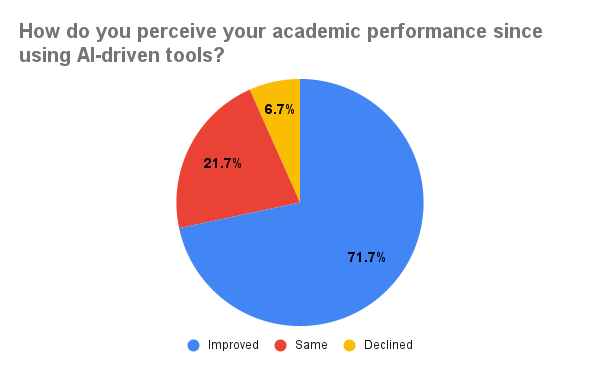
\includegraphics[width=11cm, height=7cm]{./chap4/figures/prf}
% 	\captionof{figure}{perceive academic performance using AI-driven tools}
% \end{figure}

\begin{figure}[h]
	\centering
	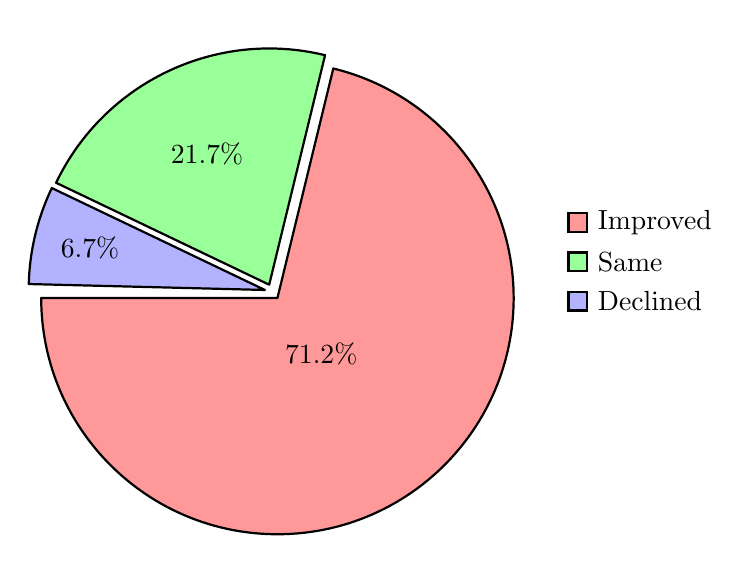
\begin{tikzpicture}
		\pie [rotate = 180, explode = 0.1, text=legend, color = {red!40, green!40, blue!30}]
		{71.2/ Improved,
			21.7/ Same,
			6.7/ Declined }
	\end{tikzpicture}
	\captionof{figure}{Perceived academic performance using AI-driven tools}
\end{figure}

After assessing the respondents' opinions on the use of AI-driven tools and students'
academic performance, it is obvious that the majority of their academic performance is improved.
The data reported that 71.7\% agreed that AI improves their academic performance.
In addition, 21.7\% of respondents believed that the use of AI did not affect their
academic performance. Whereas 6.7\% showed negative results, believing
that AI affects their academic performance to be declined while using it.
\subsection{The students' engagements while using AI-driven tools in an academic setting}

% \begin{figure}[H]
% 	\centering
% 	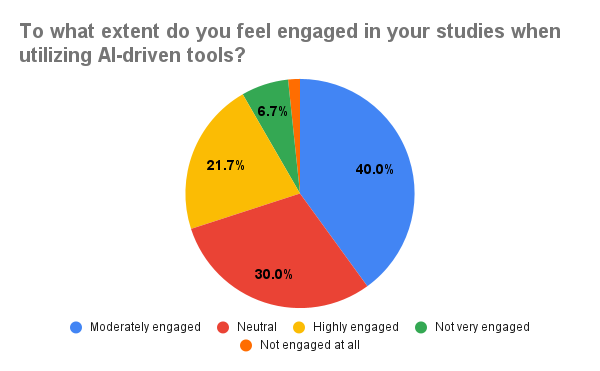
\includegraphics[width=11cm, height=7cm]{./chap4/figures/engagment}
% 	\captionof{figure}{perceive academic engagment using AI-driven tools}
% \end{figure}

\begin{figure}[H]
	\centering
	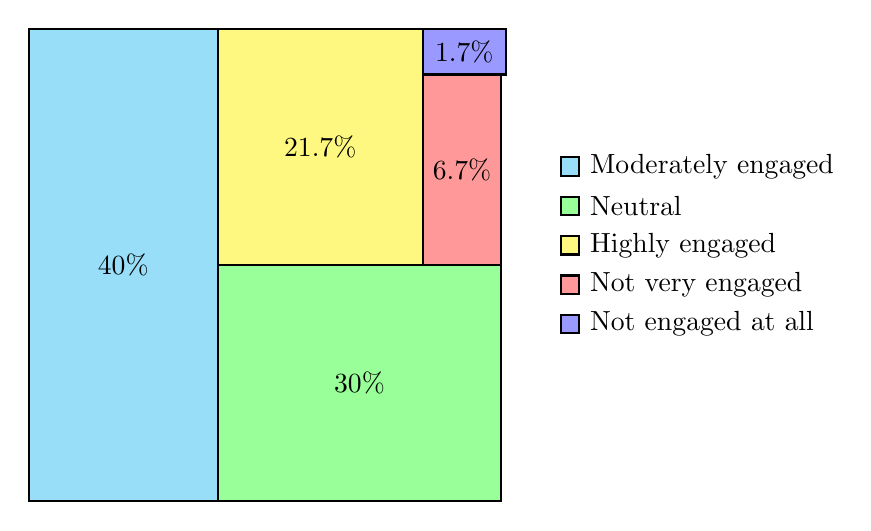
\begin{tikzpicture}
		\pie [square, text=legend, color = {cyan!40, green!40, yellow!50, red!40, blue!40}]
		{40/ Moderately engaged,
			30/ Neutral,
			21.7/ Highly engaged,
			6.7/ Not very engaged,
			1.7/ Not engaged at all }
	\end{tikzpicture}
	\captionof{figure}{Perceived academic engagement using AI-driven tools}
\end{figure}

The data collected on the extent of student engagement when using AI-driven
tools provides a diverse range of perceptions and experiences.
A significant portion of respondents reported moderately engaged, 40\%,
indicating a level of engagement with these AI-driven tools, with almost equal neutrality,
30\%, suggesting a mixed reception. However, a notable subset of students
reported feeling highly engaged 21.7\%, depicting that these tools can effectively
encourage students to be engaged.
Negatively, the presence of respondents feeling not very engaged 6.7\% and 1.7\% not
engaged at all highlights potential limitations or challenges associated with the
implementation or usage of AI-driven tools.

\subsection{Challenges faced while using AI-driven tools in academic setting}

% \begin{figure}[H]
% 	\centering
% 	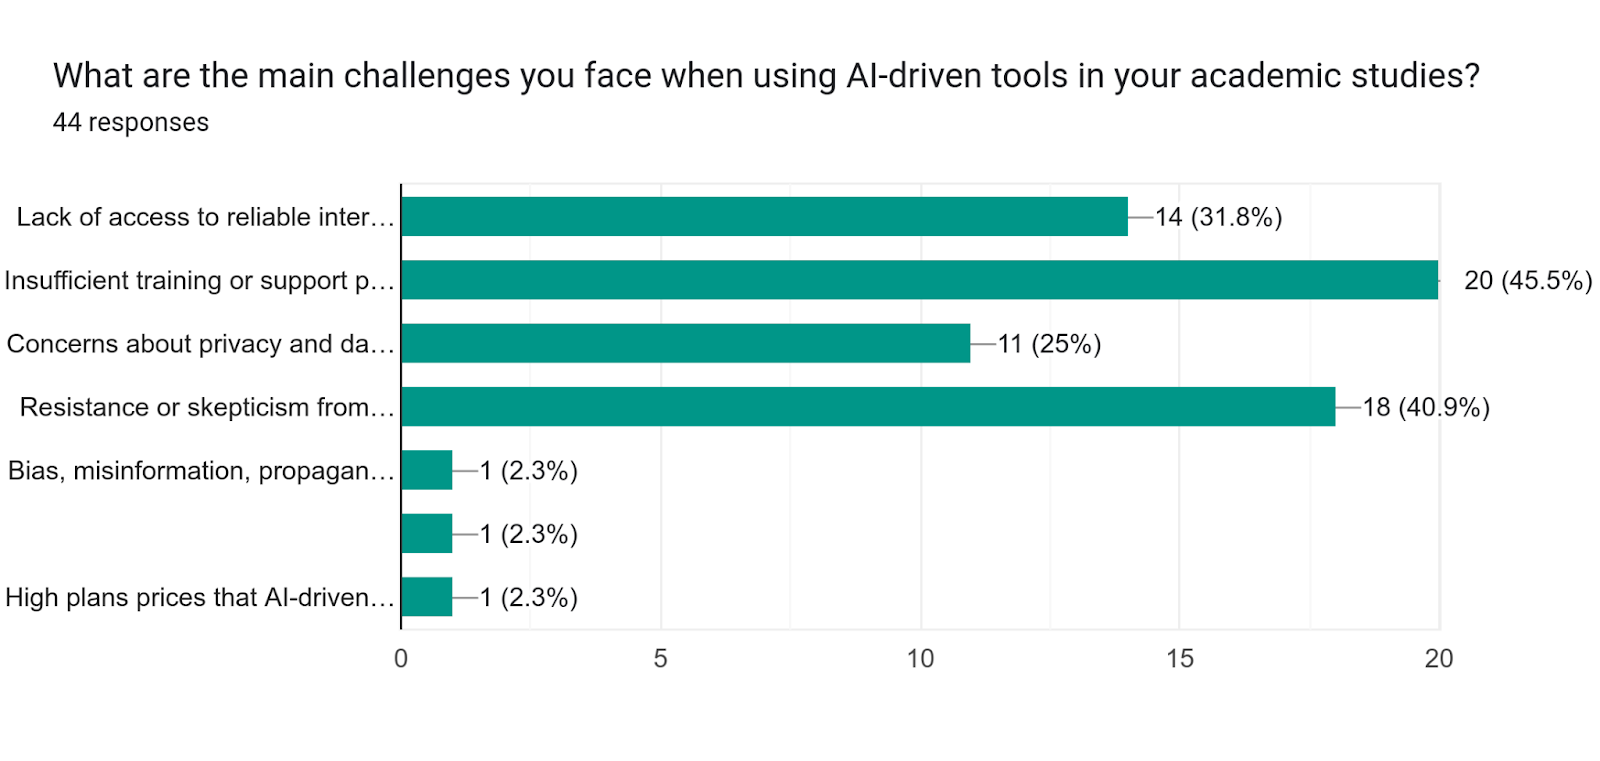
\includegraphics[width=17cm, height=9cm]{./chap4/figures/chall}
% 	\captionof{figure}{challenges faced when using AI-driven tools in academic setting}
% \end{figure}

\begin{figure}[H]
	\centering
	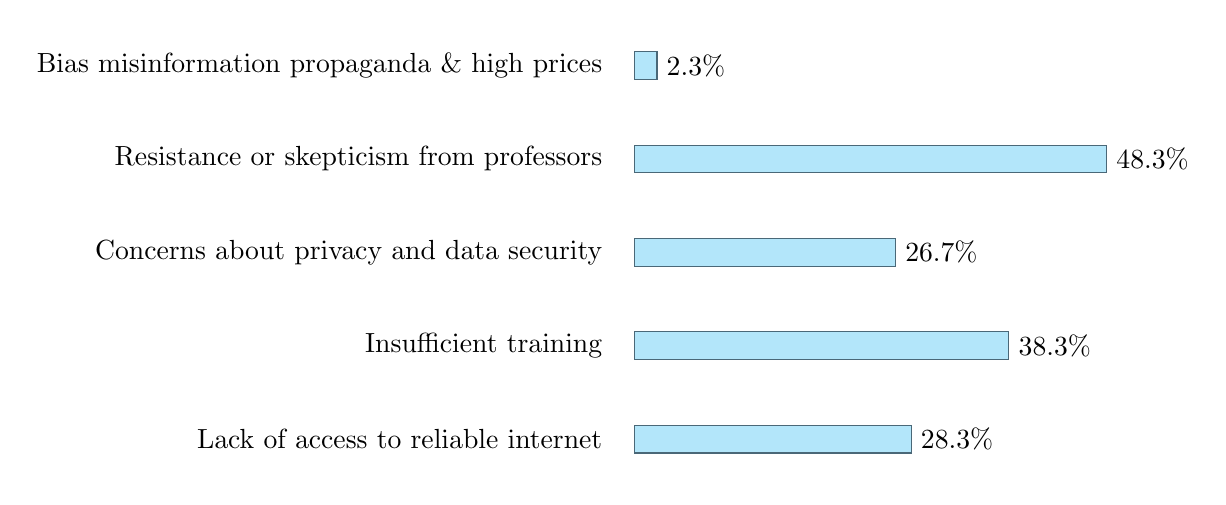
\begin{tikzpicture}
		\begin{axis}[
				xbar,
				y axis line style = { opacity = 0 },
				axis x line       = none,
				tickwidth         = 0pt,
				ytick             = data,
				enlarge y limits  = 0.1,
				symbolic y coords = {Lack of access to reliable internet, Insufficient training, Concerns about privacy and data security, Resistance or skepticism from professors, Bias misinformation propaganda \& high prices},
				nodes near coords={\pgfmathprintnumber{\pgfplotspointmeta}\%},
				nodes near coords align={horizontal},
			]
			\addplot[fill=cyan!30!white, draw=cyan!40!black] coordinates {
					(48.3,Resistance or skepticism from professors)
					(38.3,Insufficient training)
					(28.3,Lack of access to reliable internet)
					(26.7,Concerns about privacy and data security)
					(2.3,Bias misinformation propaganda \& high prices)
				};
		\end{axis}
	\end{tikzpicture}
	\captionof{figure}{challenges faced when using AI-driven tools in academic setting}
\end{figure}
The bar chart shows the results of a survey on the challenges students face when using AI-driven tools in their academic studies.
Out of 60 respondents, the biggest challenge was reported to be the resistance or skepticism from professors toward using AI-driven
tools, with 48.3\% of students selecting that option. Insufficient training is the second challenge faced by 38.8\%.
Following the lack of access to reliable internet, 28.3\% of students reported this as a challenge.
In addition, 26.7\% of students reported concern with their privacy and data security matters. At the same time,
2.3\% was bias, misinformation, propaganda in the AI tools, and high prices of the AI-driven tools.
\subsection{AI-driven tools and opportunities for improving learning experiences in the humanities }
% \begin{figure}[H]
% 	\centering
% 	\captionof{figure}{AI-driven tools and oppu}
% 	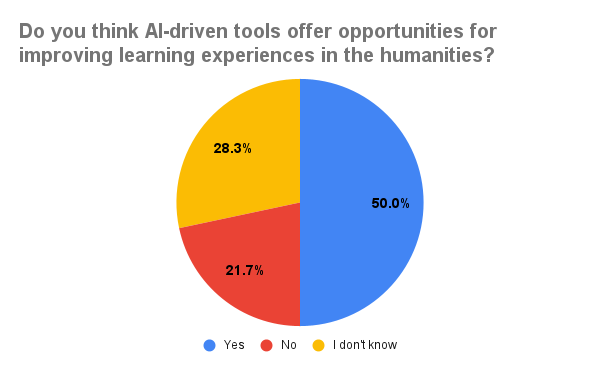
\includegraphics[width=11cm, height=7cm]{./chap4/figures/op.png}
% \end{figure}

\begin{figure}[h]
	\centering
	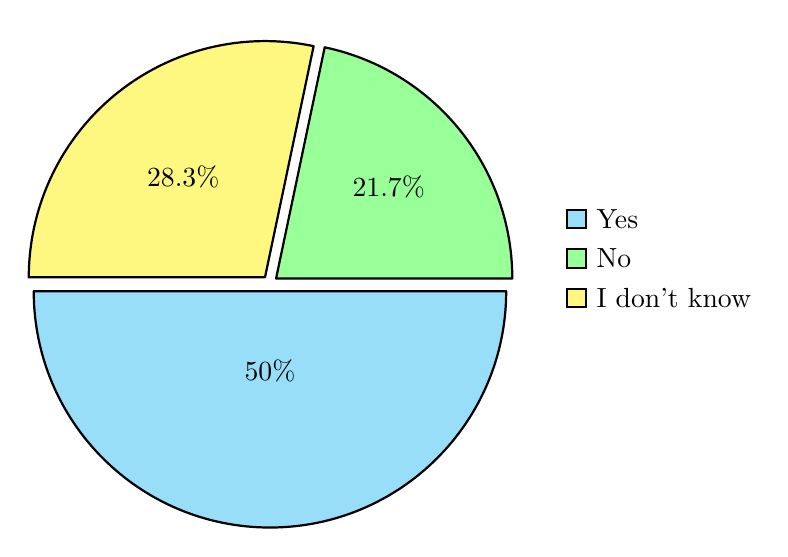
\begin{tikzpicture}
		\pie [rotate=180, explode=0.1, text=legend, color = {cyan!40, green!40, yellow!50,}]
		{
			50/ Yes,
			21.7/ No,
			28.3/ I don't know
		}
	\end{tikzpicture}
	\captionof{figure}{AI and opportunities}
\end{figure}
The majority of English university students reported that 50\% of AI-driven tools offer opportunities for enhancing learning experiences in the humanities.
In addition, 28.3\% report the ignorance of the opportunities that AI-driven tools offer.
On the other hand, 21.7\% reported that AI-driven tools offer an opportunity to enhance the learning experience within the humanities setting.

Those who answered with yes a question were asked to get some examples from students
to understand what kind of opportunities AI-driven tools can offer to enhance the learning experiences,
and the answers were follow:

% 1st resp
\resp{1}{AI-driven tools in higher education could enhance personalized learning
	through adaptive learning platforms and virtual
	tutoring, and improve research with data analysis tools.}
% 2nd resp
\resp{2}{Research Assistance: AI can assist
	researchers in analyzing vast amounts of
	data, generating hypotheses, and identifying trends,
	accelerating the pace of discovery.}
% 3rd resp
\resp{3}{It can help students be more self-reliant
	and seek knowledge wherever and whenever they want to.}
%4rd resp 
\resp{4}{Making student more used to communicate with chat
	bot ai characters when they can't find native speakers to communicate with.}
%5th resp
\resp{5}{It helps you correct some mistakes and learn from them.
	It elevates your writing and information base and limit their context.}

As it is shown the majority of english students to claim that AI-driven tools can
help students to boost their productivity through analysing the data for researcheres
and provide personalized learning through adaptive learning platforms and virtual tutoring.

\section{Discussion}
It is important to restate the current study's goals and research 
hypothesis before delving into the research findings and discussion.
As mentioned in the introduction, the primary aim of this paper is 
to assess English students' attitudes toward using AI-driven tools
to improve their academic performance and learning experiences. 
Consequently, the recent study has significantly contributed to 
validating or refuting the hypotheses stated in the previous chapter. 
These hypotheses were as follows:
\begin{itemize}
	\item AI-driven tools are singificantly fostering engagment in academic setting.
	\item AI-driven tools are significantly improving academic performance.
	\item There are challenges and opportunities are associated with using AI in higher education
	      in Morocco, specifically in the humanities
\end{itemize}
The current study's findings strongly demonstrate students' positive 
attitudes toward using AI-driven tools as learning aids. 
Precise questions were asked to explore the students' perceptions of the use of AI-driven tools.

Firstly, the findings reveal a significant 40\% 
increase in student engagement when utilizing AI technologies. 
The data collected from English university students strongly 
supports the idea that AI can effectively enhance student engagement, 
fostering a more interactive and dynamic learning environment. 
This aligns with existing literature that emphasizes 
the role of technology in promoting active participation among students.


Secondly, the research results demonstrate a positive correlation 
between using AI-driven tools and students' academic performance. 
As per the data, 71\% of participants believed that AI-driven tools improved their academic performance.
Similarly, a related study by \citep{mohammed_exploring_2023} demonstrated 
that AI-driven tools can effectively enhance academic performance and foster engagement. 
Results showed that most respondents agreed that \say{ChatGPT} motivates and 
engages students by offering access to many resources and improving academic performance.


Furthermore, the research findings shed light on students' challenges 
when utilizing AI-driven tools in educational settings. According to
the participants, these challenges offer valuable insights into the
practical obstacles associated with implementing AI technologies in
learning environments. Issues such as technical difficulties, lack
of training, resistance or skepticism of professors, and concerns
regarding data privacy and security emerge as significant hurdles
that need to be addressed to ensure the effective utilization of AI in education.


Finally, the research results highlight the opportunities presented
by AI-driven tools for transforming learning experiences in the humanities.
By exploring students' perspectives and experiences with AI technologies,
the study uncovers the potential for personalized learning, adaptive tutoring,
and data analysis to help researchers with their vast amount of data.
These opportunities align with the broader literature on the transformative
impact of AI in education, emphasizing technology's role in facilitating
innovative and tailored learning experiences. Leveraging these opportunities
can empower educators to create engaging, effective, and personalized learning
environments that cater to the diverse needs of students in the humanities.
\section{Conclusion}

Throughout this chapter, we have conducted an ongoing study related to
students' attitudes towards the use of AI-driven tools as a learning
tool to enhance learning experiences within academic settings. The
aim was to present and discuss the study's findings in depth.
In addition, this study sought to validate or reject the formulated
hypotheses mentioned in the methodology chapter, correlate the
concluded findings with the paper's literature review and see
how far it converges or diverges from it. The final chapter
will discuss the implications and the limitations of this
study. Finally, it would cover an inclusive summary of the
research paper and serve as a springboard to a more in-depth analysis.

 

\chapter{GENERAL CONCLUSION}
\section{Introduction}

This chapter offers a general overview of this research paper.
It contains a restatement of the current study’s objectives, a summary
of the methodology and findings obtained from the investigation, and 
it provides limitations and suggestions for further studies.

\section{Summary of the Research Goal}

This paper is an attempt to explore university students’ attitudes towards the 
use of AI as a tool to enhance the learning experiences within the humanities, 
namely improving academic performance and engagement. In addition, exploring the
challenges and opportunities faced by humanities students(the study focuses on English university students).

\section{Summary of the Findings}


The present study is based on quantitative and qualitative data collection. 
It indicates that Moroccan English students at the University of Hassan II and the faculty of Ben Msik have
a positive attitude towards using AI to improve their learning experiences. 
The majority of respondents believe that their academic performance has improved since using AI.
The findings suggest that AI can enhance personalized learning and enable researchers to analyze their data accurately. 
Additionally, AI helps students to remain moderately engaged in the classroom
despite challenges that may hinder their preference for using AI for academic purposes. 
These findings are consistent with previous studies and demonstrate the benefits of using AI in an academic context. 
Furthermore, the responses from participants confirmed the research hypotheses, which are:
\begin{itemize}
	
\item AI-driven tools significantly promote engagement in academic settings.
\item AI-driven tools significantly improve academic performance.
\item There are challenges and opportunities associated with using AI in higher education in Morocco, especially in the humanities.
\end{itemize}
\section{Limitations of the study}
This study investigated the feasibility of using AI-driven tools in the academic context to enhance learning experiences.
It was particularly interesting to see whether AI-driven tools promote engagement and improve academic performance.
The current research provided evidence for the effectiveness of achieving an enhanced learning experience in higher education.
 However, it is imperative to acknowledge certain limitations inherent in this study. 
Foremost, the absence of professors' perspectives constitutes a significant gap, 
given their pivotal role within the educational ecosystem. In addition,
the scope of this study does not encompass a diverse array of university 
students across different disciplines, thereby limiting the generalizability 
of its findings. To gain a more comprehensive understanding, 
it is crucial to gather additional data 
from participants across a wider range of Moroccan universities before making any generalizations.
\section{Implications of the Study}

The findings of the current study and previous research clearly demonstrate that AI can
improve learning experiences in higher education.
This can lead to increased student engagement and improved academic performance.
Given these findings, it is recommended that educators and learners incorporate this valuable
technology into teaching and learning practices. The use of AI technology can benefit humanities
students, particularly those studying English, by enhancing their listening, speaking, reading, 
and writing skills, as well as expanding their vocabulary. Additionally, educators can utilize 
AI to automate routine tasks, allowing them to focus on core objectives and deliver effective lesson plans.

\section{Suggestions for further research}

The use of AI in higher education to enhance learning experiences is a newly emerging area.
Further study will contribute to its survival and development.
Therefore, future research should broaden the scope by collecting more data 
from different universities in various regions of Morocco. 
In addition, it is important to consider the perspectives of the professors to obtain more truthful and accurate findings.

\section{Conclusion}

The 21st century has seen a technological revolution, with the widespread availability
of devices used for communication, entertainment, and education. This research paper
aims to examine the effectiveness of AI-driven tools, such as mobile and web applications,
in improving learning experiences within Moroccan higher education institutions. 
This chapter provides a conclusion to the main points explored in the study, 
including a summary of the research goals, methodology, findings, suggestions 
for further research, as well as the limitations and implications of the study.


\printbibliography[heading=bibintoc, title=REFERENCES]
\end{document}
